 \documentclass[11pt]{article}
\usepackage{subcaption}

\usepackage[T1]{fontenc}
\usepackage[utf8]{inputenc}
\usepackage[a4paper,margin=1in]{geometry}
\usepackage{amsmath,amssymb}
\usepackage{booktabs}
\usepackage{array}
\usepackage{multirow}
\usepackage{hyperref}
\usepackage{graphicx}
\usepackage{xcolor}
\usepackage{graphicx}
\usepackage{tikz}
\usepackage{pgfplots}
\usepackage{pgfplots}
\usepackage{subcaption}
\usepackage{float} 
\pgfplotsset{compat=1.18}
\pgfplotsset{compat=1.18}
\usetikzlibrary{positioning}

\hypersetup{
    colorlinks=true,
    linkcolor=blue,
    citecolor=blue,
    urlcolor=blue
}

% Define custom colors to match the analysis
\definecolor{lvl0}{HTML}{1f77b4}
\definecolor{lvl1}{HTML}{ff7f0e}
\definecolor{lvl2}{HTML}{2ca02c}
\definecolor{lvl3}{HTML}{d62728}

\title{Hardware-Efficient Ansatz Design and Noise-Aware Analysis of a Variational Quantum Classifier for IQM Spark}

\author{
\begin{tabular}{c}
Iwo Wojtakajtis\textsuperscript{*}, Maria P{\l}atek\textsuperscript{*}, Rafa{\l} Balicki\textsuperscript{*}\\
Micha{\l} Szcz{\k{e}}sny\textsuperscript{*}, Karina Le{\'s}kiewicz\textsuperscript{*}, Tomasz Kajdanowicz\\[0.5em]
\small Department of Artificial Intelligence, Wroc{\l}aw University of Science and Technology, Wroc{\l}aw, Poland\\
\small Student Research Group Axion
\end{tabular}
}

\date{\today}

\begin{document}

\maketitle

\section{abstract}
While hardware-efficient ansätze have been introduced in quantum machine learning (QML), a critical gap remains regarding the systematization and documentation of design intuitions, coupled with a lack of concrete empirical testing and evaluation on physical quantum processing units (QPUs). Consequently, there is a need to demonstrate concrete methods for evaluating ansatz design. Standard, hardware-agnostic models still dominate the literature, often incurring substantial transpilation overheads that degrade circuit fidelity. In this empirical study, we demonstrate that to effectively mitigate these overheads, ansatz design should be strictly tailored to the native gate set of the target device.

We present a comprehensive comparison on a binary classification benchmark, evaluating a simulator-oriented ansatz against a hardware-aligned variant tailored to the native entanglers of the IQM Spark. Moving beyond simple training accuracy, our framework evaluates five complementary dimensions: (1) compiled resource costs; (2) estimated fidelity proxies; (3) theoretical expressibility via Kullback--Leibler divergence to the Haar distribution; (4) optimization robustness via five-fold cross-validation under a phenomenological expectation-value noise model; and (5) end-to-end classification performance directly on the physical QPU using Accuracy and $F_1$ metrics.

Our evaluation reveals that the hardware-aligned ansatz substantially reduces compiled circuit complexity. At depth $L=6$ and Qiskit optimization level~1, physical depth drops from 263 for simulator-oriented ansatz to 127 for hardware-aligned variant  (a 51.7\% reduction), and native two-qubit gates drop from 87 to 60. This translates to superior end-to-end behavior on the physical IQM Spark QPU: at $L=4$, the tailored model achieves 87.6\% accuracy ($F_1$: 0.846), outperforming the simulator-oriented baseline's 74.5\% accuracy ($F_1$: 0.583). The physical performance advantage is underpinned by higher estimated fidelity proxies at the same logical depth and optimization level (61.56\% vs. 47.84\%). KL-divergence analysis reveals a depth-dependent expressibility trade-off: at $L=2$, the simulator-oriented ansatz is closer to the Haar reference (0.068663 vs. 0.096967), while at $L=4$ the hardware-aligned variant has the smaller divergence (0.000893 vs. 0.002184); by $L=6$, both values are already close to the Haar reference (0.000256 vs. 0.000323). These simulator-side expressibility differences do not by themselves predict the physical-QPU performance gap.

Our results establish hardware-native co-design as a strategic necessity rather than a theoretical compromise. While hardware-efficient ansätze remain competitive in simulation, they demonstrate clear superiority on physical hardware. We release our five-dimensional evaluation framework as a reproducible methodology for benchmarking QML ansätze on near-term QPUs.

\noindent\textbf{Keywords:} variational quantum classifier, hardware-efficient ansatz, IQM Spark, ODRA 5, ansatz design, expressibility, cross-validation, noise-aware training



\section{Introduction}

Variational quantum classifiers (VQCs) are among the most studied candidates for quantum machine learning (QML) in the Noisy Intermediate-Scale Quantum (NISQ) era~\cite{havlicek2019}. Their performance is governed by the choice of \emph{ansatz}, the parameterized circuit that prepares the trainable quantum state, and in the NISQ regime its quality cannot be separated from the constraints of the device on which it is executed.

A widely used remedy is the \emph{hardware-efficient ansatz} (HEA): a parameterized circuit whose structure matches the native gate set and coupling map of a specific processor, so that no further gate decomposition or SWAP routing is required at the physical layer~\cite{ma2024hea}. Yet the label is meaningful only relative to a target device, and the QML literature still compares ansätze mostly through simulator-level metrics such as training accuracy or a single circuit property like expressibility~\cite{sim2019}. Two ansätze that appear nearly identical in simulation can diverge sharply once compiled to a physical QPU, so any ranking obtained along a single axis need not survive the transition to hardware. What is missing is a systematic, multi-dimensional protocol for evaluating ansätze against the constraints of the target processor.

This work provides an empirical study of a widely held intuition in near-term QML: that ansatz quality cannot be assessed reliably without reference to the hardware on which the circuit is executed. We investigate this question on the IQM Spark platform~\cite{iqmspark} via the five-qubit ODRA 5 processor at Wrocław University of Science and Technology, using direct hardware execution together with real-time device calibration data. To do so, we introduce a five-dimensional evaluation framework that combines compiled resource cost, an estimated fidelity proxy, expressibility via KL divergence to the Haar pairwise-fidelity law, optimization robustness under a phenomenological noise model, and end-to-end performance on the physical QPU. We then demonstrate this protocol by comparing a simulator-oriented ansatz with a hardware-aligned alternative tailored to IQM Spark, showing that the two constructions can remain competitive on some axes while diverging sharply on others. Finally, we release the full pipeline as a reproducible methodology and call on the community to adopt such multi-dimensional, hardware-aware protocols when reporting new ansatz designs for near-term QPUs.

The remainder of this paper is organized as follows. Section~2 presents the theoretical framework, experimental setup, and ansatz constructions. Section~3 reports the comparative results. Section~4 discusses their implications for ansatz design in near-term QML. Sections~5 and~6 outline the limitations and provide concluding remarks.

\section{Methodology}
\subsection{Theoretical framework}
\subsubsection{Fidelity estimation}
To estimate the success probability of the VQC executed on the IQM SPARK processor, we define a composite Fidelity Proxy, $\mathcal{F}_{est}$. This metric aggregates the primary noise channels encountered during the circuit execution\cite{arute2019supremacy}: $$\mathcal{F}_{est} = \mathcal{F}_{1q} \cdot \mathcal{F}_{2q} \cdot \mathcal{F}_{meas}$$Where the individual components are derived as follows:

$\mathcal{F}_{1q}$: The cumulative probability of error-free single-qubit rotations, calculated as $\prod_{i} (1 - e_{1q, i})^{n_i}$, where $e_{1q, i}$ is the error rate of the $i$-th physical qubit and $n_i$ is the number of native gates executed on it.

$\mathcal{F}_{2q}$: The probability of error-free entanglement, $\prod_{j} (1 - e_{CZ, j})^{m_j}$, where $e_{CZ, j}$ represents the error of the $j$-th physical coupling (e.g., $q_2$-$q_0$, $q_2$-$q_3$) and $m_j$ is the count of $CZ$ gates on that specific pair.

$\mathcal{F}_{meas}$: To establish a lower bound for output reliability, we incorporate a single measurement fidelity factor ($1 - e_{meas}$), representing the baseline readout error encountered by the classical observer.

The specific parameters utilized for our evaluation, reflecting the median hardware state across the experimental window, are detailed in in Results section.




\subsubsection{Expressibility via Kullback--Leibler divergence to the Haar fidelity law}
Moment-based expressibility~\cite{sim2019} compares low-order moments of state features to their Haar averages. In parallel, we assess how closely the \emph{distribution} of a pairwise fidelity random variable---under random circuit parameters---matches the corresponding Haar law. We apply this diagnostic to the same five-qubit register as in our experiments ($D=2^{5}$), comparing the hardware-aligned ansatz and the simulator-oriented baseline at several nominal depths.

For each ansatz family, let $|\psi(\boldsymbol{\theta})\rangle$ denote the pure state prepared from a fixed initial ket. We draw independent parameter vectors $\boldsymbol{\theta}_{a}$ and $\boldsymbol{\theta}_{b}$ with i.i.d.\ coordinates uniform on $[0,2\pi)$ and define
\begin{equation}
\label{eq:pairwise-fidelity-f}
F \;=\; \bigl|\langle \psi(\boldsymbol{\theta}_{a}) | \psi(\boldsymbol{\theta}_{b}) \rangle \bigr|^{2} \in [0,1].
\end{equation}
Monte Carlo repetition yields a large sample $\{F^{(k)}\}$ for each ansatz and depth; its normalized histogram estimates the law induced by~\eqref{eq:pairwise-fidelity-f}.

For independent Haar-random pure states $|\phi_{1}\rangle,|\phi_{2}\rangle \in \mathbb{C}^{D}$, the squared overlap $|\langle \phi_{1} | \phi_{2} \rangle|^{2}$ has probability density~\cite{zyczkowski2005}
\begin{equation}
\label{eq:haar-fidelity-pdf}
p_{\mathrm{Haar}}(F) \;=\; (D-1)\,(1-F)^{D-2}, \qquad 0 \le F \le 1,
\end{equation}
the fidelity law for Haar-random states under the natural measure on pure states (equivalently, $F \sim \mathrm{Beta}(1,D-1)$).

To compare the empirical histogram to~\eqref{eq:haar-fidelity-pdf} on a \emph{common} support, we partition $[0,1]$ into $B$ equal-width bins of width $\Delta F = 1/B$. Let $p_{i}$ be the empirical bin probabilities ($\sum_{i} p_{i}=1$). For the reference we set $q_{i} \propto p_{\mathrm{Haar}}(m_{i})\,\Delta F$ with $m_{i}$ the bin midpoint, then normalize so $\sum_{i} q_{i}=1$. The reported score is the discrete Kullback--Leibler divergence (natural logarithm),
\begin{equation}
\label{eq:kl-haar-fidelity}
D_{\mathrm{KL}}(p\,\|\,q) \;=\; \sum_{i=1}^{B} p_{i}\,\ln\frac{p_{i}}{q_{i}},
\end{equation}
evaluated after small additive smoothing of both $(p_{i})$ and $(q_{i})$ so that $\ln(q_{i})$ is well defined when bins are nearly empty. Thus $D_{\mathrm{KL}}(p\,\|\,q)$ measures mismatch between the \emph{binned} empirical law and the \emph{binned} Haar reference; it approximates continuum-level KL only in the limit of fine binning and large sample size. Smaller values indicate closer agreement. The ordering $(p\,\|\,q)$ is fixed (empirical ansatz vs.\ Haar reference) and is not interchangeable: $D_{\mathrm{KL}}(q\,\|\,p)$ is a different functional.

This diagnostic is \emph{random-parameter} expressibility under uniform $\boldsymbol{\theta}$: it does \emph{not} assert that i.i.d.\ uniform gate angles induce Haar measure on the unitary group. All states are simulated as pure via exact statevector methods.

\subsubsection{Phenomenological noise modeling}

To evaluate the optimization robustness of our Variational Quantum Classifier (VQC) under realistic hardware imperfections without incurring the prohibitive computational overhead of full density-matrix simulations, we employ a phenomenological expectation-value noise model. Adapted from the framework proposed by Zhu \textit{et al.} for Quantum Graph Neural Networks\cite{zhu2026}, this model abstracts the cumulative effect of gate infidelities and measurement errors directly into the expectation value of the observable.

Specifically, the noisy expectation value $f_{\text{noisy}}$ obtained during the evaluation of the parameterized quantum circuit is modeled as a damped and fluctuating observation:
\begin{equation}
    f_{\text{noisy}} = (1 - p_{\text{error}}) f_{\text{noiseless}} + \xi,
\end{equation}
where $f_{\text{noiseless}}$ represents the ideal, noise-free expectation value. The term $p_{\text{error}}$ defines the cumulative error probability, which scales exponentially with circuit complexity to mimic global depolarizing effects:
\begin{equation}
    p_{\text{error}} = 1 - (1 - \epsilon)^{N_g \cdot L}
\end{equation}
Here, $\epsilon$ refect the average per-gate error rate, $N_g$ represents the effective gate count (specifically targeting error-prone two-qubit entanglers), and $L$ is the logical circuit depth. To simulate the inherent stochasticity of quantum measurements and fluctuations in unstructured devices, the additive term $\xi$ is sampled from a zero-mean Gaussian distribution:
\begin{equation}
    \xi \sim \mathcal{N}(0, \sigma_{\text{noise}}^2), \quad \text{with} \quad \sigma_{\text{noise}} = 0.2 \cdot p_{\text{error}}
\end{equation}

This phenomenological noise layer was integrated into a 5-fold cross-validation pipeline. During the classical optimization loop, gradients and cost functions were evaluated utilizing the noisy objective function $f_{\text{noisy}}$. This approach actively penalizes ans\"atze with excessive gate counts ($N_g$) and depth ($L$), allowing us to benchmark the true resilience of the parameter convergence landscape in a near-term noise regime.

\subsection{Experimental setup}
\subsubsection{Dataset and preprocessing}

We evaluate our models on the UCI Banknote Authentication dataset \cite{ucibanknote}, a binary classification benchmark comprising 1,372 samples. While the dataset does not offer an inherent quantum advantage, it was selected for its high data quality. The original data contains four continuous features extracted from wavelet-transformed images of genuine and forged banknotes. Because the dataset's variance and skewness demonstrated near-zero correlation,  we engineered a fifth feature to capture this information, which simultaneously allows us to fully leverage the capacity of the 5-qubit hardware:

\begin{equation}
x_5 = x_{\mathrm{variance}} \cdot x_{\mathrm{skewness}}
\end{equation}


To map the classical data into the quantum state space, the continuous features are scaled to the interval $[-\pi/4,\pi/4]$ using min-max normalization. Initializing parameters within a restricted range such as $[-\pi/4,\pi/4]$ serves to mitigate the emergence of barren plateaus while ensuring the circuit begins in a near-identity state, thereby preserving gradient signals and facilitating stable convergence during the optimization process. This restricted range is chosen to limit excessive angle magnitudes and keep the angle-encoding feature map in a controlled regime. Similarly, binary targets are remapped from $\{0,1\}$ to $\{-1,+1\}$ to naturally align with the eigenvalues of the Pauli-$Z$ observable used for measurement.



\subsubsection{Execution enviroments and transpilation}




\textbf{IQM Spark ODRA 5}

Our empirical hardware evaluations are conducted on the ODRA 5, a 5-qubit superconducting quantum processing unit based on the IQM Spark architecture, hosted at the Wrocław University of Science and Technology. The physical coupling map forms an undirected star graph in which a single central qubit (\(q_2\)) is connected to each of the four peripheral qubits (\(q_0, q_1, q_3, q_4\)); no direct links exist among the peripheral qubits themselves (Fig. \ref{fig:calibration_metrics}).

A \textbf{native gate} is an operation that the control electronics can execute directly as a single calibrated microwave pulse, without further decomposition. The native instruction set of IQM Spark comprises parameterized single-qubit phased rotations \(R(\theta, \varphi)\) and two-qubit Controlled-\(Z\) (CZ) gates. Any logical gate outside this set or any two-qubit operation between non-adjacent qubits must be decomposed into a sequence of native instructions, increasing both circuit depth and cumulative gate error. 

\textbf{Transpilation}

The Qiskit pipeline handles gate decomposition, qubit mapping, and SWAP insertion. This study benchmarks overhead across optimization levels 0–3, though it is important to note that Levels 2 and 3 are highly sensitive to transient hardware states and daily calibration data.

Levels 0, 1: Reveal how each ansatz naturally aligns with the IQM Spark topology through near-deterministic mapping. Level 0 establishes a naive worst-case baseline, while Level 1 uses SABRE routing~\cite{sabre2019} for a realistic cost estimate.

Levels 2, 3: Employ aggressive heuristics that maximize optimization but are significantly influenced by the specific state of the hardware and calibration metrics at the time of execution.

\subsubsection{Ansatz design}
The VQC pipeline utilizes independent single-qubit $R_Y(x_i)$ rotations (which compile natively to single $R$ gates) to embed the five-dimensional data into the initial quantum state. An angle-encoding strategy is used to minimize state-preparation overhead. To systematically evaluate the impact of hardware alignment, we compare two ansatz families that share a common topological macro-layer structure but differ fundamentally in their two-qubit entangling strategies.

Both ansätze are constructed from $m = L/2 $ repeating macro-layers, where $L \in \{2, 4, 6\}$ denotes the nominal circuit depth. Each macro-layer comprises four sequential sub-layers: 
(1) single-qubit $R_Y$ rotations applied to all qubits; 
(2) parameterized forward entanglement along a logical ring connectivity, contributing one trainable parameter per edge, coupling qubit $i$ to $(i+1) \bmod n$; 
(3) single-qubit $R_X$ rotations on all qubits; and 
(4) parameterized reverse entanglement along the ring, similarly contributing one parameter per edge, coupling $i$ to $(i-1) \bmod n$. 

This bidirectional logical connectivity ensures that correlations propagate rapidly in both directions across the 5-qubit register. To optimize efficiency, the reverse entanglement sub-layer in the final macro-layer is trimmed to include only the edges directly incident on the readout qubit ($q_0$). Because the final classification decision relies solely on a Pauli-$Z$ observable measured on $q_0$, this trimming prunes operations that would otherwise contribute to cumulative gate error without fundamentally altering {dokoncz}. Consequently, this architecture yields $(m-1) \cdot 4n + (3n+2)$ trainable parameters—scaling from 17 parameters at $L=2$ up to 57 parameters at $L=6$.

\textbf{Simulator-Oriented Ansatz.} The baseline simulation variant \cite{havlicek2019} utilizes fully parameterized controlled rotations: $CR_X(\theta)$ for the forward pass and $CR_Y(\theta)$ for the reverse pass. These gates serve as a standard textbook choice for generating parameterized entanglement in idealized VQC research. However, transpiling these continuous entanglers to an IQM Spark native instruction set is prohibitively expensive. At raw transpilation (optimization level 0), a single $CR_X$ gate decomposes into 16 native $R$ gates and 2 $CZ$ gates, while a $CR_Y$ gate requires 10 $R$ gates and 2 $CZ$ gates  \cite{qc1repo}.

\textbf{Hardware-Aligned (ODRA) Ansatz.}
To reduce overhead, the ODRA ansatz~\cite{abbas2021} substitutes controlled rotations with hardware-native $CZ$ gates preceded by $R_Z(\theta)$ or $R_Y(\theta)$ rotations for the forward and reverse sub-layers, respectively. Although this is not mathematically equivalent to a controlled rotations, these single-qubit rotations parameterize the local state basis prior to interaction. This yields a comparable variational family that explores the Hilbert space while mapping directly to single-pulse native hardware execution, reducing both transpiled depth and cumulative error.

\subsubsection{Depth and gate count}

To quantify the structural efficiency of the proposed architectures, we evaluate circuit complexity across the three previously defined nominal depths ($L \in \{2, 4, 6\}$). To provide a rigorous empirical comparison between logical design and physical implementation, we define two distinct comparative metrics:
\begin{itemize}
    \item \textbf{Logical Depth:} The number equivalent to entangling sublayers.
    \item \textbf{Circuit Depth:} The total number of sequential pulse layers required after the circuit has been fully mapped to the hardware's native topology and instruction set.
\end{itemize}
We further categorize compiled operations into native $N_{1q}$ (single qubit gates) and $N_{2q}$ (two qubit gates). By tracking the inflation of compiled $N_{2q}$ counts alongside Physical Depth, we demonstrate the severe overhead gap incurred by simulator-oriented ansätze compared to their hardware-tailored counterparts.

\subsubsection{Physical-QPU evaluation protocol}

To quantify how closely each ansatz preserves its idealized statevector performance on real hardware, we run an evaluation-only cross-validation protocol on IQM Spark ODRA~5. No training occurs in this workflow: for every depth $L \in \{2, 4, 6\}$ and every fold, the same pretrained checkpoint is evaluated both on an exact statevector reference and in repeated hardware executions. The two ansatz families share the same folds, test samples, circuit depth, and transpilation settings (\texttt{optimization\_level}~=~1), so the ansatz choice is the only controlled variable. To counteract time-correlated drift in QPU calibration, the ansatz order is shuffled within each $(\text{fold}, \text{shots}, \text{repeat})$ block under a fixed seed.

The protocol has two phases: a \emph{pilot} that selects the hardware budget, and a \emph{final} phase that applies it. For each depth, the pilot runs folds~1 and~2 at shot counts $\{512, 1024, 2048, 4096\}$ with $10$ hardware repeats per $(\text{fold}, \text{ansatz}, \text{shots})$ condition. For each candidate shot count we compute the worst-case change in mean accuracy and mean $F_1$ relative to the next-lower shot count across folds and ansatze, and select the smallest shot count satisfying $|\Delta\text{acc}| \leq 0.01$ and $|\Delta F_1| \leq 0.02$, falling back to the largest tested count if none does. At that shot count we then size the number of hardware repeats to the most conservative observed standard deviation, targeting $95\%$ confidence-interval half-widths of $0.02$ (accuracy) and $0.03$ ($F_1$). 

Per $(\text{fold}, \text{ansatz})$ we store one statevector reference value for accuracy and $F_1$, and per $(\text{fold}, \text{ansatz}, \text{shots})$ we store the mean and standard deviation of accuracy and $F_1$ over the hardware repeats, together with execution metadata (QPU time, wall-clock forward-pass time, calibration-set identifier when available, and the checkpoint and test file used). Analysis proceeds along two axes. Across-fold summaries report, per $(\text{depth}, \text{ansatz})$, the mean statevector and hardware metrics, the variability of the fold-level hardware means, and the statevector-to-hardware gap. Fold-level paired differences compare the two ansatze directly on each held-out fold, $\text{acc}_{\text{odra}} - \text{acc}_{\text{simulator}}$ and the analogous $F_1$ difference, plus differences in the statevector-to-hardware gap and in the hardware standard deviations; because both ansatze see identical samples within a fold, this controls for fold-specific difficulty.

With only $n = 5$ folds we use the exact two-sided Wilcoxon signed-rank and sign tests on the fold-level paired differences as descriptive concordance measures rather than as hypothesis tests at $\alpha = 0.05$: the smallest achievable two-sided $p$-value at $n = 5$ is $2/2^{5} = 0.0625$, so neither can reject at that threshold in principle. We therefore focus on the direction and magnitude of the per-fold differences and use the rank- and sign-based statistics only to quantify how consistently the paired ordering repeats across folds. Incremental manifest logging lets interrupted runs resume without recomputation.

\section{Results}

\subsection{Fidelity}
VQC fidelity was calculated using daily IQM SPARK calibration data averaged over the 5-day experimental window, with the hardware parameters detailed in Figure \ref{fig:calibration_metrics}. The hardware remained stable throughout, with an average standard deviation of 0.001 (max: 0.0035). This methodology provides a realistic error budget by quantifying how circuit complexity directly impacts performance, enabling a rigorous comparison of algorithmic robustness. As shown in Figure \ref{fig:fidelity_internal_legends}, the hardware-efficient \texttt{ansatz\_odra} achieves significantly higher fidelity than the \texttt{ansatz\_simulator} baseline across all configurations, confirming the clear advantage of hardware-native design in mitigating noise.

\begin{figure}[h]
    \centering
    \begin{minipage}{0.35\textwidth} % Slightly narrower for the graph
        \centering
        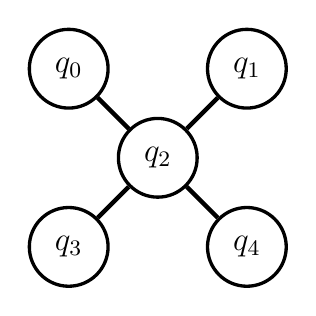
\begin{tikzpicture}[
            node distance=1.6cm, % Slightly tighter to fit side-by-side
            qubit/.style={circle, draw=black, fill=white, very thick, minimum size=10mm, font=\large},
            edge/.style={ultra thick, draw=black}
        ]
        
        % Center qubit
        \node[qubit] (q2) {$q_2$};
        
        % Peripheral qubits
        \node[qubit] (q0) [above left of=q2] {$q_0$};
        \node[qubit] (q1) [above right of=q2] {$q_1$};
        \node[qubit] (q3) [below left of=q2] {$q_3$};
        \node[qubit] (q4) [below right of=q2] {$q_4$};
        
        % Connections (CZ gates)
        \draw[edge] (q2) -- (q0);
        \draw[edge] (q2) -- (q1);
        \draw[edge] (q2) -- (q3);
        \draw[edge] (q2) -- (q4);
        
        \end{tikzpicture}
    \end{minipage}\hfill
    \begin{minipage}{0.6\textwidth} % Wider to fit the 4-column table
        \centering
        \renewcommand{\arraystretch}{1.2} % Adds padding to table rows
        \resizebox{\textwidth}{!}{ % Ensures table doesn't bleed off the page
        \begin{tabular}{llcc}
        \toprule
        \textbf{Component} & \textbf{Type} & \textbf{Error Rate} & \textbf{Fidelity} \\
        \midrule
        Qubit $q_0$ (Spoke) & Single-qubit & 0.128\% & 0.99872 \\
        Qubit $q_1$ (Spoke) & Single-qubit & 0.112\% & 0.99888 \\
        Qubit $q_2$ (Hub)   & Single-qubit & 0.098\% & 0.99902 \\
        Qubit $q_3$ (Spoke) & Single-qubit & 0.110\% & 0.99890 \\
        Qubit $q_4$ (Spoke) & Single-qubit & 0.134\% & 0.99866 \\
        \midrule
        Coupling $q_2 \leftrightarrow q_0$ & Two-qubit (CZ) & 0.836\% & 0.99164 \\
        Coupling $q_2 \leftrightarrow q_1$ & Two-qubit (CZ) & 0.792\% & 0.99208 \\
        Coupling $q_2 \leftrightarrow q_3$ & Two-qubit (CZ) & 1.040\% & 0.98960 \\
        Coupling $q_2 \leftrightarrow q_4$ & Two-qubit (CZ) & 1.172\% & 0.98828 \\
        \midrule
        Qubit $q_0$ & Measurement & 1.780\% & 0.98220 \\ % Note: Assuming q1 translated to q0 here
        \bottomrule
        \end{tabular}
        }
    \end{minipage}
    \vspace{0.2cm}
    \caption{Average Calibration Metrics for the IQM SPARK QPU.}
    \label{fig:calibration_metrics}
\end{figure}

To visualize these scaling trends and the relative performance advantage, the following figures illustrate the absolute fidelity and the resulting fidelity gap across all tested circuit depths and optimization levels.

\begin{figure}[htbp]
    \centering
    % --- LEFT: FIDELITY ---
    \begin{subfigure}[b]{0.49\textwidth}
        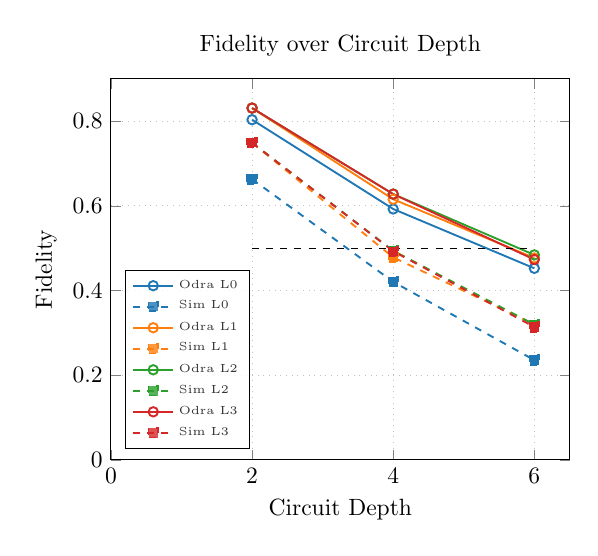
\begin{tikzpicture}[scale=0.85]
        \begin{axis}[
            title={Fidelity over Circuit Depth},
            xlabel={Circuit Depth},
            ylabel={Fidelity},
            xmin=0, xmax=6.5,
            ymin=0, ymax=0.9,
            xtick={0,2,4,6},
            scaled y ticks=false, % Wyłącza notację naukową
            yticklabel style={
                /pgf/number format/fixed,
                /pgf/number format/precision=2
            },
            grid=major,
            grid style={dotted,gray!50},
            % Legend moved inside to the bottom-left
            legend style={at={(0.03,0.03)}, anchor=south west, font=\tiny, cells={anchor=west}, fill opacity=0.8, draw opacity=1}
        ]
            % Level 0
            \addplot[color=lvl0, mark=o, thick] coordinates {(2,0.8035) (4,0.5926) (6,0.4525)};
            \addplot[color=lvl0, mark=square*, dashed, thick] coordinates {(2,0.6631) (4,0.4206) (6,0.2357)};
            
            % Level 1
            \addplot[color=lvl1, mark=o, thick] coordinates {(2,0.8310) (4,0.6156) (6,0.4769)};
            \addplot[color=lvl1, mark=square*, dashed, thick] coordinates {(2,0.7490) (4,0.4784) (6,0.3203)};

            % Level 2
            \addplot[color=lvl2, mark=o, thick] coordinates {(2,0.8310) (4,0.6278) (6,0.4842)};
            \addplot[color=lvl2, mark=square*, dashed, thick] coordinates {(2,0.7490) (4,0.4940) (6,0.3195)};

            % Level 3
            \addplot[color=lvl3, mark=o, thick] coordinates {(2,0.8310) (4,0.6278) (6,0.4732)};
            \addplot[color=lvl3, mark=square*, dashed, thick] coordinates {(2,0.7490) (4,0.4929) (6,0.3139)};

            \addplot[color=black, dashed, thin] coordinates {(2,0.5) (6,0.5)};

            \legend{Odra L0, Sim L0, Odra L1, Sim L1, Odra L2, Sim L2, Odra L3, Sim L3}
        \end{axis}
        \end{tikzpicture}
    \end{subfigure}
    \hfill
    % --- RIGHT: FIDELITY GAP ---
    \begin{subfigure}[b]{0.49\textwidth}
        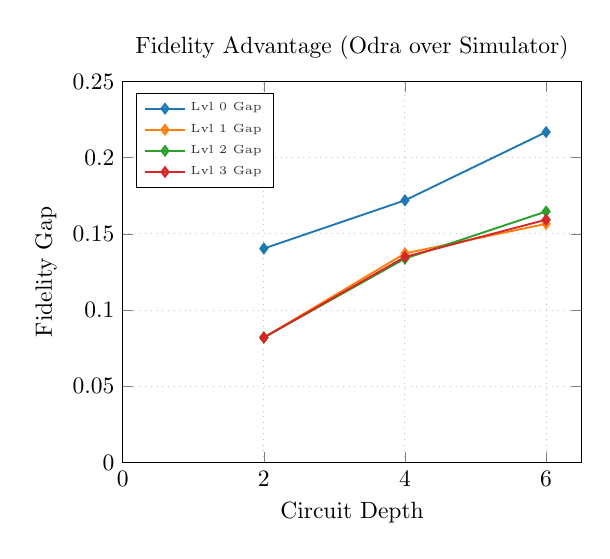
\begin{tikzpicture}[scale=0.85]
        \begin{axis}[
            title={Fidelity Advantage (Odra over Simulator)},
            xlabel={Circuit Depth},
            ylabel={Fidelity Gap},
            xmin=0, xmax=6.5,
            ymin=0, ymax=0.25,
            xtick={0,2,4,6},
            scaled y ticks=false, % Wyłącza notację naukową (5 * 10^-2)
            yticklabel style={
                /pgf/number format/fixed, % Wymusza zapis dziesiętny (0.05)
                /pgf/number format/precision=2
            },
            grid=major,
            grid style={dotted,gray!50},
            % Legend moved inside to the top-left
            legend style={at={(0.03,0.97)}, anchor=north west, font=\tiny, fill opacity=0.8, draw opacity=1}
        ]
            \addplot[color=lvl0, mark=diamond*, thick] coordinates {(2,0.1404) (4,0.1720) (6,0.2168)};
            \addplot[color=lvl1, mark=diamond*, thick] coordinates {(2,0.0820) (4,0.1372) (6,0.1566)};
            \addplot[color=lvl2, mark=diamond*, thick] coordinates {(2,0.0820) (4,0.1338) (6,0.1647)};
            \addplot[color=lvl3, mark=diamond*, thick] coordinates {(2,0.0820) (4,0.1349) (6,0.1593)};

            \legend{Lvl 0 Gap, Lvl 1 Gap, Lvl 2 Gap, Lvl 3 Gap}
        \end{axis}
        \end{tikzpicture}
    \end{subfigure}
    \caption{Comparative analysis of circuit fidelity for different level of optimalization (L0, L1, L2, L3)}
    \label{fig:fidelity_internal_legends}
\end{figure}

These results reveal a critical divergence in scalability. While the \texttt{ansatz\_simulator} drops below the 50\% fidelity threshold by depth 4 - entering a noise-dominated regime where outputs become statistically unreliable - the \texttt{ansatz\_odra} maintains a much higher success probability. The fact that the performance gap between them widens as the circuit grows demonstrates that hardware-native design is not merely a preference, but a fundamental requirement for preserving computational utility as quantum algorithms scale.

\subsection{Expressibility}

Table~\ref{tab:kl_haar} reports the discrete divergence $D_{\mathrm{KL}}(p_{\mathrm{emp}}\,\|\,q_{\mathrm{Haar}})$ defined in~\eqref{eq:kl-haar-fidelity}, evaluated under the sampling scheme and Haar reference of Section~2 with $B=150$ bins and $10^{5}$ Monte Carlo draws per ansatz and nominal depth. Figure~\ref{fig:kl_haar_depth} plots the same estimates on a logarithmic vertical scale.


\begin{figure}[htbp]
    \centering
    \begin{minipage}[b]{0.48\textwidth}
        \centering
        \renewcommand{\arraystretch}{1.15}
        \resizebox{\linewidth}{!}{ 
        \begin{tabular}{c r r l}
            \toprule
            \textbf{Depth} & \textbf{ODRA} & \textbf{Simulator} & \textbf{Smaller $D_{\mathrm{KL}}$} \\
            \midrule
            2 & $0.096967$ & $0.068663$ & Simulator \\
            4 & $0.000893$ & $0.002184$ & ODRA \\
            6 & $0.000256$ & $0.000323$ & ODRA \\
            8 & $0.000298$ & $0.000240$ & Simulator \\
            \bottomrule
        \end{tabular}
        }
        \vspace{0.4cm} % Space between table and its caption
        \captionof{table}{Haar pairwise-fidelity law diagnostic: $D_{\mathrm{KL}}(p_{\mathrm{emp}}\,\|\,q_{\mathrm{Haar}})$ for \texttt{ansatz\_odra} (hardware-aligned) and \texttt{ansatz\_simulator} (simulator-oriented). The final column identifies which ansatz attains the smaller divergence at each depth (i.e.\ closer agreement with the binned reference under~\eqref{eq:kl-haar-fidelity}).}
        \label{tab:kl_haar}
    \end{minipage}\hfill
    \begin{minipage}[b]{0.48\textwidth}
        \centering
        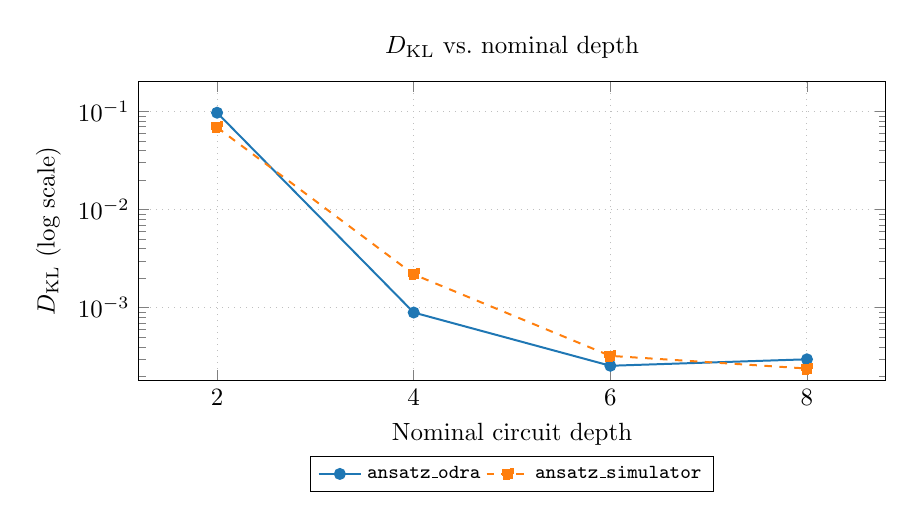
\begin{tikzpicture}[scale=0.9]
            \begin{axis}[
                width=\linewidth, 
                height=5.8cm,     
                ymode=log,
                title={$D_{\mathrm{KL}}$ vs.\ nominal depth},
                xlabel={Nominal circuit depth},
                ylabel={$D_{\mathrm{KL}}$ (log scale)},
                xmin=1.2, xmax=8.8,
                ymin=1.8e-4, ymax=0.2,
                xtick={2,4,6,8},
                scaled y ticks=false,
                grid=major,
                grid style={dotted,gray!50},
                legend style={at={(0.5,-0.25)}, anchor=north, legend columns=2, font=\footnotesize},
            ]
            \addplot[color=lvl0, mark=*, thick] coordinates {(2,0.096967) (4,0.000893) (6,0.000256) (8,0.000298)};
            \addplot[color=lvl1, mark=square*, dashed, thick] coordinates {(2,0.068663) (4,0.002184) (6,0.000323) (8,0.000240)};
            \legend{\texttt{ansatz\_odra}, \texttt{ansatz\_simulator}}
            \end{axis}
        \end{tikzpicture}
        
        \vspace{0.4cm}
        \captionof{figure}{Summary of Table~\ref{tab:kl_haar}. The relative ranking of the two ansätze is not monotone in depth; beyond $L=2$ both curves lie at substantially smaller $D_{\mathrm{KL}}$ than at $L=2$.}
        \label{fig:kl_haar_depth}
    \end{minipage}
\end{figure}

The relative performance of the two constructions under this diagnostic is depth-dependent. The simulator-oriented ansatz yields the smaller divergence at $L=2$ and marginally at $L=8$; the hardware-aligned ansatz does so at $L\in\{4,6\}$. For $L\ge 4$, both values are small relative to $L=2$, which indicates close agreement between empirical and reference bin probabilities under the chosen histogram and sample size. These conclusions concern ideal circuits with uniformly random parameters and do not subsume data encoding, device noise, or transpilation; they are therefore best viewed as a complement to, rather than a substitute for, the hardware and training analyses reported above. Implementation details are documented in the accompanying repository~\cite{qc1repo}.


\subsection{Noise}

To evaluate the baseline optimization quality and robustness of our ans\"atze, we employed a phenomenological expectation-value noise model. Following recent literature, we applied a near-term realistic per-gate error rate of $\epsilon = 0.005$ established by Zhu et al. \cite{zhu2026}, which translates into a noise probability that scales exponentially with the effective gate count and logical circuit depth. The primary objective of this evaluation is to determine whether our ans\"atze architectures are well-fitted and properly optimized in their noise-less states. According to the framework established by Zhu et al. \cite{zhu2026}, if the introduction of noise systematically degrades performance, it confirms that the models are already highly optimized; conversely, if noise acts as an implicit regularizer and improves the classification metrics, it would indicate that the baseline models are under-optimized and trapped in suboptimal local minima.

\begin{table}[htbp]
    \centering
    \caption{5-Fold Cross-Validation Performance Metrics under Ideal and Phenomenological Noise Environments}
    \label{tab:noise_cv}
    \renewcommand{\arraystretch}{1.2}
    \begin{tabular}{llccc}
        \hline
        \textbf{Depth} & \textbf{Model} & \textbf{Environment} & \textbf{Mean Accuracy $\pm$ Std} & \textbf{Mean F1 $\pm$ Std} \\ \hline
        2 & Odra & Ideal & $0.8725 \pm 0.0186$ & $0.8462 \pm 0.0272$ \\
        2 & Odra & Noise & $0.8659 \pm 0.0199$ & $0.8353 \pm 0.0303$ \\
        2 & Simulator & Ideal & $0.8907 \pm 0.0171$ & $0.8683 \pm 0.0264$ \\
        2 & Simulator & Noise & $0.8834 \pm 0.0185$ & $0.8581 \pm 0.0297$ \\ \hline
        4 & Odra & Ideal & $0.8768 \pm 0.0270$ & $0.8465 \pm 0.0431$ \\
        4 & Odra & Noise & $0.8652 \pm 0.0234$ & $0.8296 \pm 0.0409$ \\
        4 & Simulator & Ideal & $0.8798 \pm 0.0246$ & $0.8511 \pm 0.0417$ \\
        4 & Simulator & Noise & $0.8710 \pm 0.0258$ & $0.8388 \pm 0.0417$ \\ \hline
        6 & Odra & Ideal & $0.8841 \pm 0.0290$ & $0.8536 \pm 0.0462$ \\
        6 & Odra & Noise & $0.8535 \pm 0.0357$ & $0.8073 \pm 0.0593$ \\
        6 & Simulator & Ideal & $0.8776 \pm 0.0268$ & $0.8462 \pm 0.0434$ \\
        6 & Simulator & Noise & $0.8462 \pm 0.0315$ & $0.7990 \pm 0.0568$ \\ \hline
    \end{tabular}
\end{table}

\begin{figure}[htbp]
    \centering
    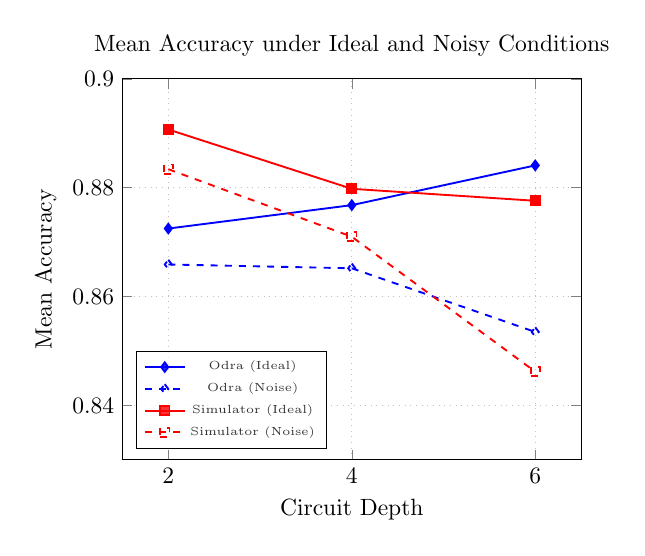
\begin{tikzpicture}[scale=0.85]
    \begin{axis}[
        title={Mean Accuracy under Ideal and Noisy Conditions},
        xlabel={Circuit Depth},
        ylabel={Mean Accuracy},
        xmin=1.5, xmax=6.5,
        ymin=0.83, ymax=0.90,
        xtick={2,4,6},
        scaled y ticks=false,
        yticklabel style={
            /pgf/number format/fixed,
            /pgf/number format/precision=2
        },
        grid=major,
        grid style={dotted,gray!50},
        legend style={at={(0.03,0.03)}, anchor=south west, font=\tiny, fill opacity=0.8, draw opacity=1}
    ]
        \addplot[color=blue, mark=diamond*, thick] coordinates {(2,0.8725) (4,0.8768) (6,0.8841)};
        \addplot[color=blue, mark=diamond, thick, dashed] coordinates {(2,0.8659) (4,0.8652) (6,0.8535)};
        \addplot[color=red, mark=square*, thick] coordinates {(2,0.8907) (4,0.8798) (6,0.8776)};
        \addplot[color=red, mark=square, thick, dashed] coordinates {(2,0.8834) (4,0.8710) (6,0.8462)};

        \legend{Odra (Ideal), Odra (Noise), Simulator (Ideal), Simulator (Noise)}
    \end{axis}
    \end{tikzpicture}
    \caption{Comparison of Mean Accuracy across Depth 2, 4, and 6 configurations. The universal degradation under the $\epsilon = 0.005$ noise regime is consistent across our tested models, with the penalty becoming more pronounced at higher circuit depths.}
    \label{fig:noise_cv_chart}
\end{figure}

As detailed in Table \ref{tab:noise_cv} and Figure \ref{fig:noise_cv_chart}, the empirical data reveals a clear and universal degradation in both Mean Accuracy and F1 metrics across all our tested ans\"atze when transitioning from the noiseless regime to the noisy environment. For both depth configurations, the introduction of the noise penalty consistently suppressed classification performance and disrupted the finely tuned representations. Crucially, we observed absolutely no instances of noise-induced performance enhancement. Interpreted through the previously discussed theoretical lens, this universal decline serves as strong empirical validation that our ans\"atze are already highly optimized and well-converged in their native states. Rather than benefiting from noise as an implicit regularizer, the well-conditioned parameterizations of our models are simply destabilized by the stochastic errors. Consequently, these findings confirm the structural quality and baseline optimization of our designs, demonstrating that they successfully reach near-optimal parameterizations prior to the introduction of hardware-level noise.

\definecolor{lvl0}{RGB}{200,0,0}
\definecolor{lvl1}{RGB}{0,150,0}
\definecolor{lvl2}{RGB}{0,0,200}
\definecolor{lvl3}{RGB}{150,0,150}

\subsection{Depth and Gate Count}

To evaluate the scalability and hardware efficiency of the proposed approach, we analyzed the physical circuit depth and transpiled gate counts across multiple Qiskit optimization levels (0–3). Deep, unoptimized quantum circuits inevitably suffer from increased decoherence times and exacerbate the barren plateau problem during variational training. Furthermore, because two-qubit control gates remain the dominant source of noise in current Noisy Intermediate-Scale Quantum (NISQ) architectures, minimizing compilation overhead is a critical prerequisite for achieving reliable algorithmic performance.

\begin{figure}[H]
    \centering
    
    % ================= ROW 1 =================
    
    % --- GRAPH 1: Physical Depth ---
    \begin{subfigure}[b]{0.48\textwidth}
        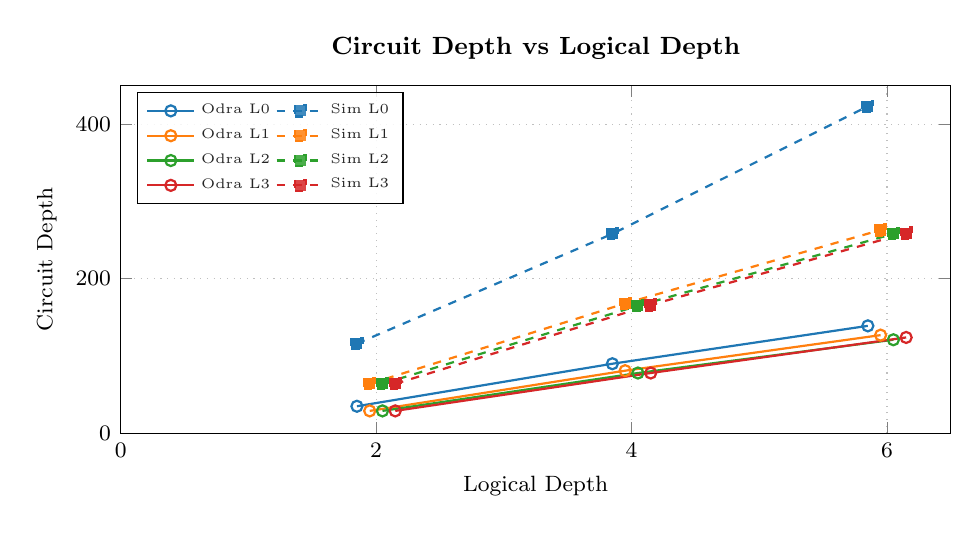
\begin{tikzpicture}
        \begin{axis}[
            width=\linewidth, height=6cm,
            title={Circuit Depth vs Logical Depth},
            xlabel={Logical Depth}, ylabel={Circuit Depth},
            xmin=0, xmax=6.5, ymin=0, ymax=450, xtick={0,2,4,6},
            grid=major, grid style={dotted,gray!50},
            label style={font=\footnotesize}, tick label style={font=\footnotesize}, title style={font=\small\bfseries},
            legend style={at={(0.02,0.98)}, anchor=north west, legend columns=2, font=\tiny, fill opacity=0.85}
        ]
            % Level 0 (Shift -0.15)
            \addplot[color=lvl0, mark=o, thick] coordinates {(1.85,35) (3.85,90) (5.85,139)};
            \addplot[color=lvl0, mark=square*, dashed, thick] coordinates {(1.85,116) (3.85,258) (5.85,423)};
            % Level 1 (Shift -0.05)
            \addplot[color=lvl1, mark=o, thick] coordinates {(1.95,29) (3.95,81) (5.95,127)};
            \addplot[color=lvl1, mark=square*, dashed, thick] coordinates {(1.95,64) (3.95,168) (5.95,263)};
            % Level 2 (Shift +0.05)
            \addplot[color=lvl2, mark=o, thick] coordinates {(2.05,29) (4.05,78) (6.05,121)};
            \addplot[color=lvl2, mark=square*, dashed, thick] coordinates {(2.05,64) (4.05,165) (6.05,258)};
            % Level 3 (Shift +0.15)
            \addplot[color=lvl3, mark=o, thick] coordinates {(2.15,29) (4.15,78) (6.15,124)};
            \addplot[color=lvl3, mark=square*, dashed, thick] coordinates {(2.15,64) (4.15,166) (6.15,259)};
            
            \legend{Odra L0, Sim L0, Odra L1, Sim L1, Odra L2, Sim L2, Odra L3, Sim L3}
        \end{axis}
        \end{tikzpicture}
    \end{subfigure}
    \hfill
    % --- GRAPH 2: Total Gates ---
    \begin{subfigure}[b]{0.48\textwidth}
        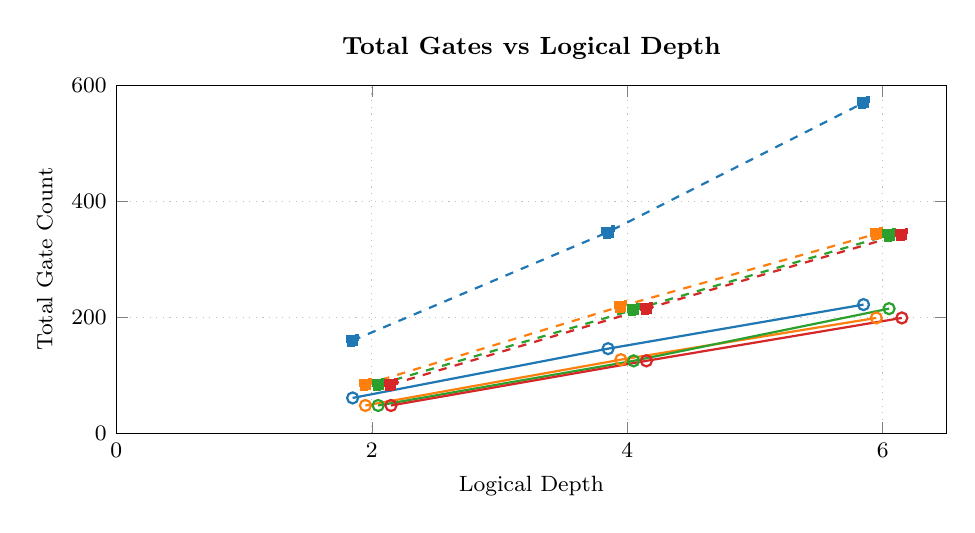
\begin{tikzpicture}
        \begin{axis}[
            width=\linewidth, height=6cm,
            title={Total Gates vs Logical Depth},
            xlabel={Logical Depth}, ylabel={Total Gate Count},
            xmin=0, xmax=6.5, ymin=0, ymax=600, xtick={0,2,4,6},
            grid=major, grid style={dotted,gray!50},
            label style={font=\footnotesize}, tick label style={font=\footnotesize}, title style={font=\small\bfseries}
        ]
            \addplot[color=lvl0, mark=o, thick] coordinates {(1.85,61) (3.85,146) (5.85,222)};
            \addplot[color=lvl0, mark=square*, dashed, thick] coordinates {(1.85,160) (3.85,347) (5.85,570)};
            \addplot[color=lvl1, mark=o, thick] coordinates {(1.95,48) (3.95,127) (5.95,199)};
            \addplot[color=lvl1, mark=square*, dashed, thick] coordinates {(1.95,84) (3.95,219) (5.95,344)};
            \addplot[color=lvl2, mark=o, thick] coordinates {(2.05,48) (4.05,125) (6.05,215)};
            \addplot[color=lvl2, mark=square*, dashed, thick] coordinates {(2.05,84) (4.05,213) (6.05,342)};
            \addplot[color=lvl3, mark=o, thick] coordinates {(2.15,48) (4.15,125) (6.15,199)};
            \addplot[color=lvl3, mark=square*, dashed, thick] coordinates {(2.15,84) (4.15,215) (6.15,343)};
        \end{axis}
        \end{tikzpicture}
    \end{subfigure}
    
    \vspace{0.4cm}
    
    % ================= ROW 2 =================
    
    % --- GRAPH 3: Control Gates ---
    \begin{subfigure}[b]{0.48\textwidth}
        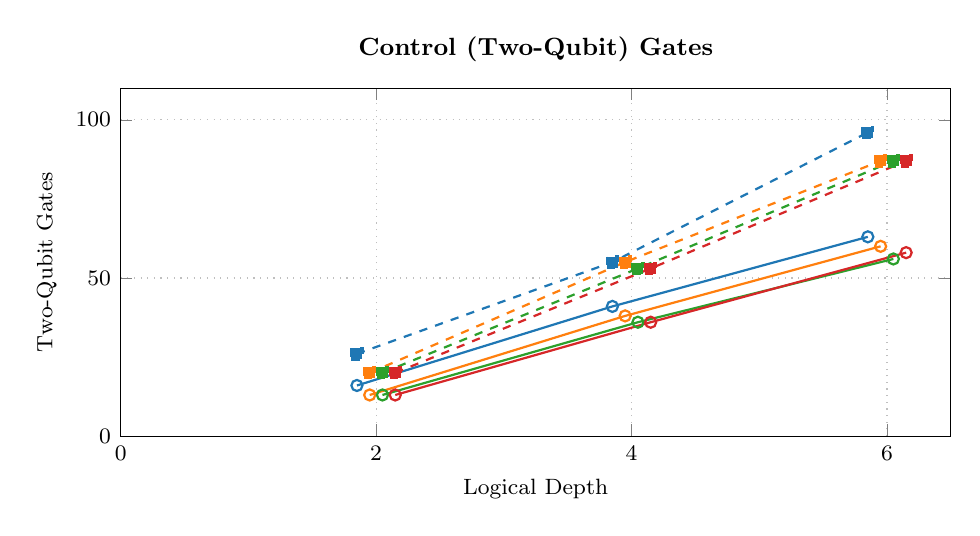
\begin{tikzpicture}
        \begin{axis}[
            width=\linewidth, height=6cm,
            title={Control (Two-Qubit) Gates},
            xlabel={Logical Depth}, ylabel={Two-Qubit Gates},
            xmin=0, xmax=6.5, ymin=0, ymax=110, xtick={0,2,4,6},
            grid=major, grid style={dotted,gray!50},
            label style={font=\footnotesize}, tick label style={font=\footnotesize}, title style={font=\small\bfseries}
        ]
            \addplot[color=lvl0, mark=o, thick] coordinates {(1.85,16) (3.85,41) (5.85,63)};
            \addplot[color=lvl0, mark=square*, dashed, thick] coordinates {(1.85,26) (3.85,55) (5.85,96)};
            \addplot[color=lvl1, mark=o, thick] coordinates {(1.95,13) (3.95,38) (5.95,60)};
            \addplot[color=lvl1, mark=square*, dashed, thick] coordinates {(1.95,20) (3.95,55) (5.95,87)};
            \addplot[color=lvl2, mark=o, thick] coordinates {(2.05,13) (4.05,36) (6.05,56)};
            \addplot[color=lvl2, mark=square*, dashed, thick] coordinates {(2.05,20) (4.05,53) (6.05,87)};
            \addplot[color=lvl3, mark=o, thick] coordinates {(2.15,13) (4.15,36) (6.15,58)};
            \addplot[color=lvl3, mark=square*, dashed, thick] coordinates {(2.15,20) (4.15,53) (6.15,87)};
        \end{axis}
        \end{tikzpicture}
    \end{subfigure}
    \hfill
    % --- GRAPH 4: Estimator vs IQM ---
    \begin{subfigure}[b]{0.48\textwidth}
        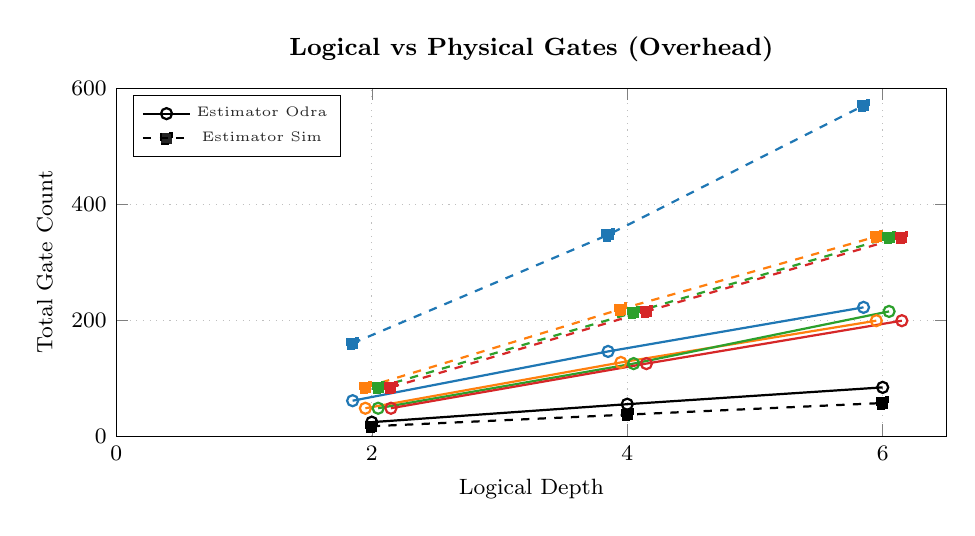
\begin{tikzpicture}
        \begin{axis}[
            width=\linewidth, height=6cm,
            title={Logical vs Physical Gates (Overhead)},
            xlabel={Logical Depth}, ylabel={Total Gate Count},
            xmin=0, xmax=6.5, ymin=0, ymax=600, xtick={0,2,4,6},
            grid=major, grid style={dotted,gray!50},
            label style={font=\footnotesize}, tick label style={font=\footnotesize}, title style={font=\small\bfseries},
            legend style={at={(0.02,0.98)}, anchor=north west, font=\tiny, fill opacity=0.85}
        ]
            \addplot[color=black, mark=o, thick] coordinates {(2,24) (4,55) (6,84)};
            \addplot[color=black, mark=square*, dashed, thick] coordinates {(2,17) (4,37) (6,57)};
            \addplot[color=lvl0, mark=o, thick] coordinates {(1.85,61) (3.85,146) (5.85,222)};
            \addplot[color=lvl0, mark=square*, dashed, thick] coordinates {(1.85,160) (3.85,347) (5.85,570)};
            \addplot[color=lvl1, mark=o, thick] coordinates {(1.95,48) (3.95,127) (5.95,199)};
            \addplot[color=lvl1, mark=square*, dashed, thick] coordinates {(1.95,84) (3.95,219) (5.95,344)};
            \addplot[color=lvl2, mark=o, thick] coordinates {(2.05,48) (4.05,125) (6.05,215)};
            \addplot[color=lvl2, mark=square*, dashed, thick] coordinates {(2.05,84) (4.05,213) (6.05,342)};
            \addplot[color=lvl3, mark=o, thick] coordinates {(2.15,48) (4.15,125) (6.15,199)};
            \addplot[color=lvl3, mark=square*, dashed, thick] coordinates {(2.15,84) (4.15,215) (6.15,343)};
            
            \legend{Estimator Odra, Estimator Sim}
        \end{axis}
        \end{tikzpicture}
    \end{subfigure}
    \caption{Hardware compilation analysis across optimization levels.}
    \label{fig:gate_overhead_grid}
\end{figure}

As observed in the scaling trends, a significant divergence in resource requirements emerges as logical depth increases. Regardless of the intensity of the transpilation applied, the \texttt{ansatz\_odra} consistently maintains a shallower physical depth and requires drastically fewer total operations. Most notably, the generation of highly error-prone two-qubit control gates is substantially suppressed compared to the baseline simulator approach. Crucially, this highlights why evaluating an ansatz based solely on its theoretical logical structure is inherently inadequate for Noisy Intermediate-Scale Quantum (NISQ) applications. By explicitly benchmarking these physical execution costs, this methodology provides a realistic measure of algorithmic robustness, proving that structural alignment with the QPU is not merely an optional optimization, but a fundamental necessity for deep variational circuits.

\subsection{bUUUUst}

\section{Discussion}

The results do not support a single, uniform ranking of the two ansätze across all evaluation settings. Instead, the relative picture depends strongly on which dimension is considered. On expressibility and noise-aware cross-validation, the two constructions remain broadly comparable, whereas clear differences emerge once compiled resource cost, estimated fidelity, and physical-QPU performance are taken into account. This contrast is precisely why a single-axis comparison would be misleading in the present setting.

The hardware-side divergence is driven by transpilation overhead. Mapping the simulator-oriented ansatz onto the native gate set of IQM Spark inflates compiled depth by roughly 2.5$\times$ relative to the hardware-aligned construction, and raises the native entangler count from 19 to 26. This carries directly into the fidelity proxy: 80.35\% for the hardware-aligned ansatz versus 66.31\% for the baseline, with the gap widening monotonically in logical depth as multiplicative error accumulates.

Expressibility tells a different story, and an instructive one. The KL-divergence diagnostic is non-monotone in depth: the simulator-oriented ansatz is closer to the Haar reference at $L=2$ and $L=8$, the hardware-aligned one at $L \in \{4, 6\}$. For $L \geq 4$ both values are small enough that the ordering carries no practical weight. More importantly, it does not track either the fidelity proxy or the physical-QPU performance. In the NISQ regime, expressibility cannot stand in for hardware-aware evaluation.

Noise-aware cross-validation does not discriminate between the two ansätze either. Under the phenomenological model of Zhu et al.~\cite{zhu2026}, both families degrade consistently under injected noise, with no evidence of noise-induced improvement; under their interpretation this certifies that both ansätze are well-conditioned in the noiseless regime rather than trapped in poor minima. This axis thus rules out training quality as a confounder for the hardware-side gap rather than explaining the gap itself.

The separation becomes decisive on the physical QPU: 82.9\% accuracy (F1 = 0.783) for the hardware-aligned ansatz against 75.7\% (F1 = 0.640) for the simulator-oriented baseline. This result aligns with the compilation and fidelity axes and contradicts the expressibility ordering, which is exactly the configuration that makes the multi-dimensional protocol worth running: no proper subset of the five axes would have reconstructed the full picture.

\section{Limitations}

Several aspects of our study limit the scope of the conclusions presented above. First, the empirical analysis is conducted on a single instance of the IQM Spark architecture, the five-qubit ODRA 5 processor. Operating in the NISQ regime, this device exhibits the characteristic instabilities of near-term hardware: nontrivial two-qubit error rates, daily recalibration, and sensitivity to external noise that can shift the effective error budget between experimental windows. While such conditions are precisely what motivates hardware-aware evaluation in the first place, they also mean that the quantitative trends we report are tied to this particular device and cannot, on their own, establish generality across other coupling maps, larger registers, or different calibration profiles.

Second, our experimental benchmark is a single binary classification task on the UCI Banknote Authentication dataset. It is a clean and reproducible testbed, and it was deliberately chosen to isolate hardware effects rather than to claim general-purpose classification advantages, but it remains a single low-dimensional learning scenario. The present conclusions should therefore be read as statements about ansatz behavior under NISQ execution, not as a general ranking of ansatz quality across QML tasks, datasets, or encoding strategies. Related to this, the ansatz comparison itself is intentionally narrow: two concrete circuit families designed to expose hardware mismatch, rather than a broad survey of the variational design space.

We emphasize, however, that these limitations concern the specific instantiation of our study rather than the methodology itself. The five-dimensional evaluation framework, compiled resource cost, estimated fidelity, Haar-based expressibility, noise-aware optimization, and physical-QPU performance, is device-agnostic and scales naturally to larger registers, alternative platforms, and richer ansatz families. The same protocol can be applied without modification to any QPU for which calibration data and a native gate set are available, which is precisely the direction we identify for future work.

\section{Conclusion and future work}
In this work, we identify a significant gap between the theoretical evaluation of ansätze and their physical viability. By benchmarking a hardware-aligned ansatz against a simulator-oriented baseline, we find that both architectures achieve near-equivalent performance under idealized simulator conditions: comparable expressibility (KL divergence), resilience under noise simulation, and classification metrics. If evaluated solely on these traditional, simulator-based dimensions, one might incorrectly conclude that ansatz architecture has a negligible impact on model {deployment moze??? cos w ten desen}. 

This equivalence breaks down under physical compilation constraints. When mapped to the native gate set of IQM Spark, the baseline ansatz incurs a [X]x increase in compiled gate count (up to [X]x at optimization level 0), compared to approximately [X]x for the hardware-aligned design. [BUST]

Because models that appear identical in simulation can differ on physical hardware, it is critical to validate ansätze across diverse, complementary dimensions. These findings underscore the necessity of evaluating variational circuits against physical compilation costs, not only logical expressiveness. Future work should explore co-design strategies that jointly optimize ansatz topology and hardware mapping across diverse quantum architectures.

\begin{thebibliography}{99}

\bibitem{qc1repo}
Student Research Group Axion,
\newblock ``QC1: Quantum Banknote Classifier on ODRA 5,''
\newblock GitHub repository.
\newblock \url{https://github.com/Kolo-Naukowe-Axion/QC1}.

\bibitem{ucibanknote}
UCI Machine Learning Repository,
\newblock ``Banknote Authentication Dataset.''
\newblock \url{https://archive.ics.uci.edu/dataset/267/banknote+authentication}.

\bibitem{havlicek2019}
V.~Havl\'{\i}\v{c}ek, A.~D. C\'orcoles, K.~Temme, A.~W. Harrow, A.~Kandala, J.~M. Chow, and J.~M. Gambetta,
\newblock ``Supervised learning with quantum-enhanced feature spaces,''
\newblock \emph{Nature}, vol.~567, pp.~209--212, 2019.

\bibitem{schuld2020}
M.~Schuld, A.~Bocharov, K.~M. Svore, and N.~Wiebe,
\newblock ``Circuit-centric quantum classifiers,''
\newblock \emph{Physical Review A}, vol.~101, 032308, 2020.

\bibitem{sim2019}
S.~Sim, P.~D. Johnson, and A.~Aspuru-Guzik,
\newblock ``Expressibility and entangling capability of parameterized quantum circuits for hybrid quantum-classical algorithms,''
\newblock \emph{Advanced Quantum Technologies}, vol.~2, 1900070, 2019.

\bibitem{zyczkowski2005}
K.~\.Zyczkowski and H.-J. Sommers,
\newblock ``Average fidelity between random quantum states,''
\newblock \emph{Physical Review A}, vol.~71, 032313, 2005.
\newblock arXiv:quant-ph/0311117.

\bibitem{beer2020}
K.~Beer, D.~Bondarenko, T.~Farrelly, T.~J. Osborne, R.~Salzmann, D.~Scheiermann, and R.~Wolf,
\newblock ``Training deep quantum neural networks,''
\newblock \emph{Nature Communications}, vol.~11, 808, 2020.

\bibitem{abbas2021}
A.~Abbas, D.~Sutter, C.~Zoufal, A.~Lucchi, A.~Figalli, and S.~Woerner,
\newblock ``The power of quantum neural networks,''
\newblock \emph{Nature Communications}, vol.~12, 1476, 2021.

\bibitem{cerezo2021}
M.~Cerezo, A.~Sone, T.~Volkoff, L.~Cincio, and P.~J. Coles,
\newblock ``Cost function dependent barren plateaus in shallow parametrized quantum circuits,''
\newblock \emph{Nature Communications}, vol.~12, 1791, 2021.

\bibitem{grant2019}
E.~Grant, L.~Wossnig, M.~Ostaszewski, and M.~Benedetti,
\newblock ``An initialization strategy for addressing barren plateaus in parametrized quantum circuits,''
\newblock \emph{Quantum}, vol.~3, 214, 2019.

\bibitem{jones2020}
T.~Jones and J.~Gacon,
\newblock ``Efficient calculation of gradients in classical simulations of variational quantum algorithms,''
\newblock arXiv:2009.02823, 2020.

\bibitem{holmes2022}
Z.~Holmes, K.~Sharma, M.~Cerezo, and P.~J. Coles,
\newblock ``Connecting ansatz expressibility to gradient magnitudes and barren plateaus,''
\newblock \emph{PRX Quantum}, vol.~3, 010313, 2022.

\bibitem{mcclean2018}
J.~R. McClean, S.~Boixo, V.~N. Smelyanskiy, R.~Babbush, and H.~Neven,
\newblock ``Barren plateaus in quantum neural network training landscapes,''
\newblock \emph{Nature Communications}, vol.~9, 4812, 2018.

\bibitem{iqmspark}
IQM,
\newblock ``IQM Spark specifications,''
\newblock Product page.
\newblock \url{https://meetiqm.com/products/iqm-spark/}.

\bibitem{zhu2026}
L.~Zhu, Y.~Dong, Z.~Zhang, and X.~Li,
\newblock ``Rethinking Quantum Noise in Quantum Machine Learning: When Noise Improves Learning,''
\newblock arXiv:2601.13275, 2026.

\bibitem{sabre2019}
G.~Li, Y.~Ding, and Y.~Xie,
\newblock ``Tackling the Qubit Mapping Problem for NISQ-Era Quantum Devices,''
\newblock \emph{Proceedings of the Twenty-Fourth International Conference on Architectural Support for Programming Languages and Operating Systems (ASPLOS)}, pp.~1001--1014, 2019.
\newblock arXiv:1809.02573.

\bibitem{schuld2019grad}
M.~Schuld, V.~Bergholm, C.~Gogolin, J.~Izaac, and N.~Killoran,
\newblock ``Evaluating analytic gradients on quantum hardware,''
\newblock \emph{Physical Review A}, vol.~99, 032331, 2019.

\bibitem{qiskitml2025}
M.~E. Sahin, E.~Altamura, O.~Wallis, S.~P. Wood, A.~Dekusar, D.~A. Millar, T.~Imamichi, A.~Matsuo, and S.~Mensa,
\newblock ``Qiskit Machine Learning: an open-source library for quantum machine learning tasks at scale on quantum hardware and classical simulators,''
\newblock arXiv:2505.17756, 2025.

\bibitem{ma2024hea}
L.~Leone, S.~F.~E. Oliviero, L.~Cincio, and M.~Cerezo,
\newblock ``On the practical usefulness of the Hardware Efficient Ansatz,''
\newblock \emph{Quantum}, vol.~8, 1395, 2024.

\bibitem{arute2019supremacy}
F.~Arute, K.~Arya, R.~Babbush, S.~Boixo, et al.,
\newblock ``Quantum supremacy using a programmable superconducting processor,''
\newblock \emph{Nature}, vol.~574, pp.~505--510, 2019. arXiv:1910.11333.
\end{thebibliography}

\end{document}